\documentclass{article}
\usepackage{amsmath}
\usepackage{amssymb}
\usepackage{fancyhdr}
\usepackage{tikz}
\usepackage{graphicx} % 1. Load the graphicx package

\usepackage[left=1in, right=1in, top=1.5in, bottom=1in]{geometry}% Set up custom header
\pagestyle{fancy}
\fancyhf{} % Clear all header and footer fields
\fancyhead[L]{Your Name} % Left header with name
\fancyhead[R]{August 26th 2025} % Right header with date
\renewcommand{\headrulewidth}{0.4pt} % Horizontal line below the header

\begin{document}

% Main title
\begin{center}
    \Large \textbf{Math 115E Activity 1} \\
    \vspace{0.2cm}
    \normalsize Chapter 1 Section 2 \\
    \normalsize Representing Collections of Numbers
\end{center}
\vspace{1cm} % Add space between the title and the first exercise

\section*{How to use Interval Notation}

\begin{figure}[h!]
    \begin{minipage}{0.48\textwidth}
        \centering
        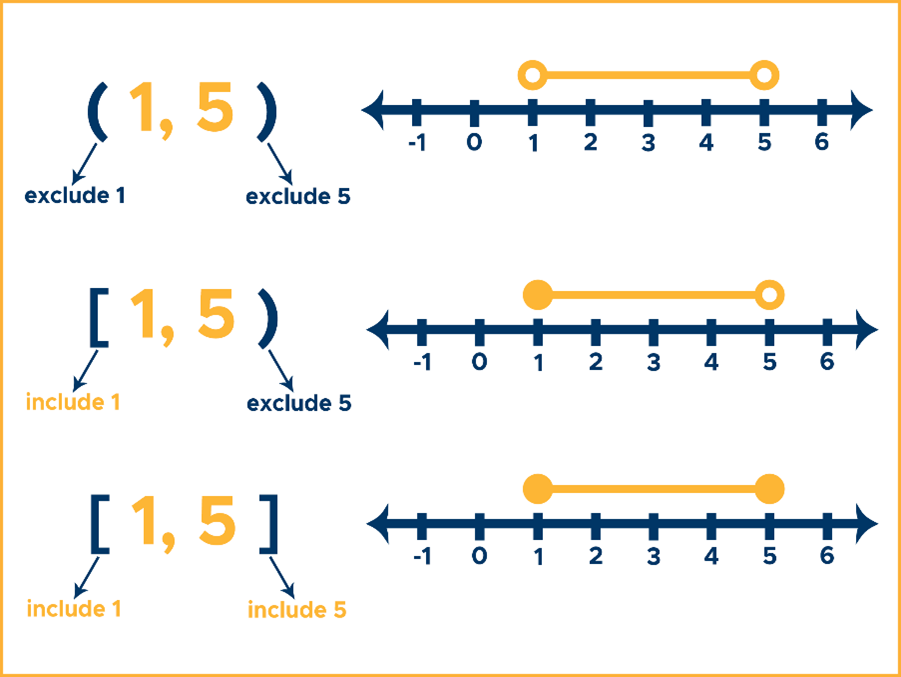
\includegraphics[scale=0.75]{Interval_chart.png}
        \label{fig:image1}
    \end{minipage}
    \hfill
    \begin{minipage}{0.48\textwidth}
        \centering
        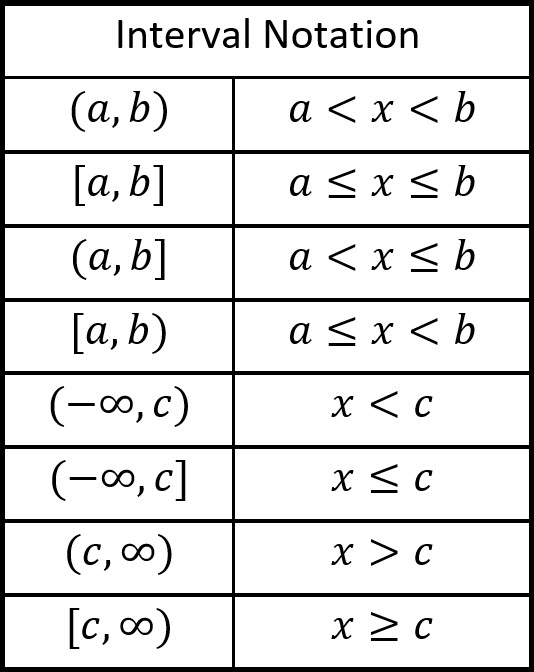
\includegraphics[scale=0.5]{Interval_chart2.jpg}
        \label{fig:image2}
    \end{minipage}
\end{figure}

% Exercise 2
\section*{Practice Problems}
In this section you will fill in the blank with a parenthesis or a bracket given the bound on the number line
\begin{enumerate}
    \item 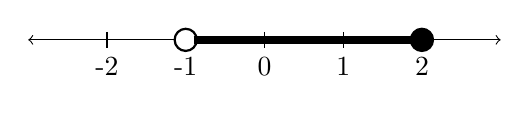
\begin{tikzpicture}
            % Draw the number line
            \draw[<->] (-3,0) -- (3,0);
            \foreach \x in {-2,-1,0,1,2}
            \draw (\x, 0.1) -- (\x, -0.1) node[below] {\x};

            % Draw the open circle at -1
            \draw[fill=white, thick] (-1,0) circle (4pt);
            % Draw the closed circle at 2
            \draw[fill=black, thick] (2,0) circle (4pt);

            % Draw the line segment between the two points
            \draw[black, line width=3pt] (-0.9,0) -- (2,0);        \end{tikzpicture}
        \rule[-8pt]{0.75pt}{8ex} \: \raisebox{-4pt}{\framebox[6mm]{\rule{0pt}{8mm}}}{\huge \,$-1, 2$ }\raisebox{-4pt}{\framebox[6mm]{\rule{0pt}{8mm}}} \: \rule[-8pt]{0.75pt}{8ex} {\huge \, $-1$}\raisebox{-4pt}{\framebox[6mm]{\rule{0pt}{8mm}}}{\huge $x$}\raisebox{-4pt}{\framebox[6mm]{\rule{0pt}{8mm}}}{\huge  $2$}
    % DONE 1 ^   
    \vspace{0.5cm}
    \item 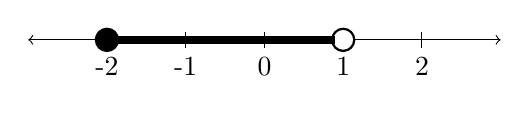
\begin{tikzpicture}
            % Draw the number line
            \draw[<->] (-3,0) -- (3,0);
            \foreach \x in {-2,-1,0,1,2}
            \draw (\x, 0.1) -- (\x, -0.1) node[below] {\x};

            % Draw the open circle at -1
            \draw[fill=black, thick] (-2,0) circle (4pt);
            % Draw the closed circle at 2
            \draw[fill=white, thick] (1,0) circle (4pt);

            % Draw the line segment between the two points
            \draw[black, line width=3pt] (-2,0) -- (0.9,0);        \end{tikzpicture}
        \rule[-8pt]{0.75pt}{8ex} \: \raisebox{-4pt}{\framebox[6mm]{\rule{0pt}{8mm}}}{\huge \,$-2, 1$ }\raisebox{-4pt}{\framebox[6mm]{\rule{0pt}{8mm}}} \: \rule[-8pt]{0.75pt}{8ex} {\huge \, $-2$}\raisebox{-4pt}{\framebox[6mm]{\rule{0pt}{8mm}}}{\huge $x$}\raisebox{-4pt}{\framebox[6mm]{\rule{0pt}{8mm}}}{\huge  $1$}
    % DONE 2 ^   
    \vspace{0.5cm}
    \item 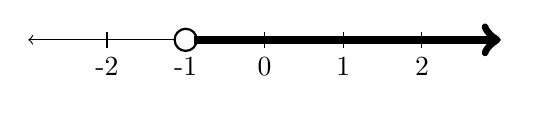
\begin{tikzpicture}
            % Draw the number line
            \draw[<->] (-3,0) -- (3,0);
            \foreach \x in {-2,-1,0,1,2}
            \draw (\x, 0.1) -- (\x, -0.1) node[below] {\x};

            % Draw the open circle at -1
            \draw[fill=white, thick] (-1,0) circle (4pt);

            % Draw the line segment between the two points
            \draw[black, line width=3pt, ->] (-0.9,0) -- (3,0);        \end{tikzpicture}
            \rule[-8pt]{0.75pt}{8ex} \: \raisebox{-4pt}{\framebox[6mm]{\rule{0pt}{8mm}}}{\huge \,$-1, \infty$ }\raisebox{-4pt}{\framebox[6mm]{\rule{0pt}{8mm}}} \: \rule[-8pt]{0.75pt}{8ex} {\huge \, $-1$}\raisebox{-4pt}{\framebox[6mm]{\rule{0pt}{8mm}}}{\huge $x$}\raisebox{-4pt}{\framebox[6mm]{\rule{0pt}{8mm}}}{\huge $\infty$}            
    % DONE 3 ^   
    \vspace{0.5cm}
    \item 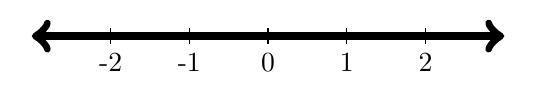
\begin{tikzpicture}
            % Draw the number line
            \draw[<->] (-3,0) -- (3,0);
            \foreach \x in {-2,-1,0,1,2}
            \draw (\x, 0.1) -- (\x, -0.1) node[below] {\x};

            % Draw the line segment between the two points
            \draw[black, line width=3pt, <->] (-3,0) -- (3,0);        \end{tikzpicture}
            \rule[-8pt]{0.75pt}{8ex} \: \raisebox{-4pt}{\framebox[6mm]{\rule{0pt}{8mm}}}{\huge \,$-\infty, \infty$ }\raisebox{-4pt}{\framebox[6mm]{\rule{0pt}{8mm}}} \: \rule[-8pt]{0.75pt}{8ex} {\huge \, $-\infty$}\raisebox{-4pt}{\framebox[6mm]{\rule{0pt}{8mm}}}{\huge $x$}\raisebox{-4pt}{\framebox[6mm]{\rule{0pt}{8mm}}}{\huge $\infty$}            
    % DONE 4 ^      
    \vspace{0.5cm}
    \item 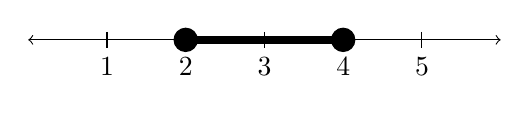
\begin{tikzpicture}
            % Draw the number line
            \draw[<->] (0,0) -- (6,0);
            \foreach \x in {1,2,3,4,5}
            \draw (\x, 0.1) -- (\x, -0.1) node[below] {\x};

            % Draw the open circle at -1
            \draw[fill=black, thick] (2,0) circle (4pt);
            % Draw the closed circle at 2
            \draw[fill=black, thick] (4,0) circle (4pt);

            % Draw the line segment between the two points
            \draw[black, line width=3pt] (2,0) -- (4,0);        \end{tikzpicture}
            \rule[-8pt]{0.75pt}{8ex} \: \raisebox{-4pt}{\framebox[36mm]{\rule{0pt}{10mm}}} \: \rule[-8pt]{0.75pt}{8ex} \: \raisebox{-4pt}{\framebox[36mm]{\rule{0pt}{10mm}}}
    % DONE 5 ^    
    \vspace{0.5cm}
    \item 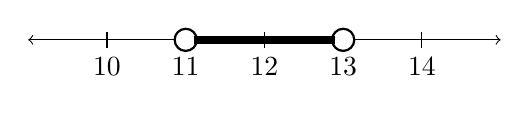
\begin{tikzpicture}
            % Draw the number line
            \draw[<->] (9,0) -- (15,0);
            \foreach \x in {10,11,12,13,14}
            \draw (\x, 0.1) -- (\x, -0.1) node[below] {\x};

            % Draw the open circle at -1
            \draw[fill=white, thick] (11,0) circle (4pt);
            % Draw the closed circle at 2
            \draw[fill=white, thick] (13,0) circle (4pt);

            % Draw the line segment between the two points
            \draw[black, line width=3pt] (11.1,0) -- (12.9,0);        \end{tikzpicture}
            \rule[-8pt]{0.75pt}{8ex} \: \raisebox{-4pt}{\framebox[36mm]{\rule{0pt}{10mm}}} \: \rule[-8pt]{0.75pt}{8ex} \: \raisebox{-4pt}{\framebox[36mm]{\rule{0pt}{10mm}}}            
    \vspace{0.5cm}
    % DONE 6 ^ 
    \item 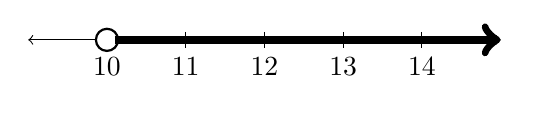
\begin{tikzpicture}
            % Draw the number line
            \draw[<->] (9,0) -- (15,0);
            \foreach \x in {10,11,12,13,14}
            \draw (\x, 0.1) -- (\x, -0.1) node[below] {\x};

            % Draw the open circle at -1
            \draw[fill=white, thick] (10,0) circle (4pt);

            % Draw the line segment between the two points
            \draw[black, line width=3pt,->] (10.1,0) -- (15,0);        \end{tikzpicture}
            \rule[-8pt]{0.75pt}{8ex} \: \raisebox{-4pt}{\framebox[36mm]{\rule{0pt}{10mm}}} \: \rule[-8pt]{0.75pt}{8ex} \: \raisebox{-4pt}{\framebox[36mm]{\rule{0pt}{10mm}}}            
    \vspace{0.5cm}
    % DONE 7 ^ 
    \item 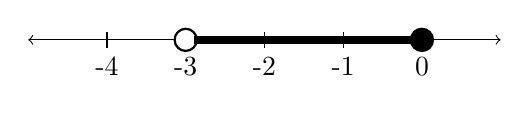
\begin{tikzpicture}
            % Draw the number line
            \draw[<->] (-5,0) -- (1,0);
            \foreach \x in {-4,-3,-2,-1,0}
            \draw (\x, 0.1) -- (\x, -0.1) node[below] {\x};

            % Draw the open circle at -1
            \draw[fill=white, thick] (-3,0) circle (4pt);
            % Draw the closed circle at 2
            \draw[fill=black, thick] (0,0) circle (4pt);

            % Draw the line segment between the two points
            \draw[black, line width=3pt] (-2.9,0) -- (0.1,0);        \end{tikzpicture}
            \rule[-8pt]{0.75pt}{8ex} \: \raisebox{-4pt}{\framebox[36mm]{\rule{0pt}{10mm}}} \: \rule[-8pt]{0.75pt}{8ex} \: \raisebox{-4pt}{\framebox[36mm]{\rule{0pt}{10mm}}}    \vspace{0.5cm}
    % DONE 8 ^ 
    \vspace{0.5cm}
    \item 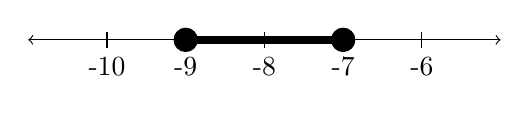
\begin{tikzpicture}
            % Draw the number line
            \draw[<->] (-11,0) -- (-5,0);
            \foreach \x in {-10,-9,-8,-7,-6}
            \draw (\x, 0.1) -- (\x, -0.1) node[below] {\x};

            % Draw the open circle at -1
            \draw[fill=black, thick] (-9,0) circle (4pt);
            % Draw the closed circle at 2
            \draw[fill=black, thick] (-7,0) circle (4pt);

            % Draw the line segment between the two points
            \draw[black, line width=3pt] (-8.9,0) -- (-6.9,0);        \end{tikzpicture}
            \rule[-8pt]{0.75pt}{8ex} \: \raisebox{-4pt}{\framebox[36mm]{\rule{0pt}{10mm}}} \: \rule[-8pt]{0.75pt}{8ex} \: \raisebox{-4pt}{\framebox[36mm]{\rule{0pt}{10mm}}}            
    % DONE 9 ^ 
    \vspace{0.5cm}
    \item 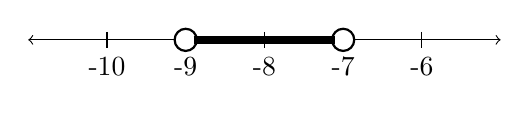
\begin{tikzpicture}
            % Draw the number line
            \draw[<->] (-11,0) -- (-5,0);
            \foreach \x in {-10,-9,-8,-7,-6}
            \draw (\x, 0.1) -- (\x, -0.1) node[below] {\x};

            % Draw the open circle at -1
            \draw[fill=white, thick] (-9,0) circle (4pt);
            % Draw the closed circle at 2
            \draw[fill=white, thick] (-7,0) circle (4pt);

            % Draw the line segment between the two points
            \draw[black, line width=3pt] (-8.9,0) -- (-7.1,0);        \end{tikzpicture}
            \rule[-8pt]{0.75pt}{8ex} \: \raisebox{-4pt}{\framebox[36mm]{\rule{0pt}{10mm}}} \: \rule[-8pt]{0.75pt}{8ex} \: \raisebox{-4pt}{\framebox[36mm]{\rule{0pt}{10mm}}}            
    % DONE 10 ^ 
    \vspace{0.5cm}
    \item 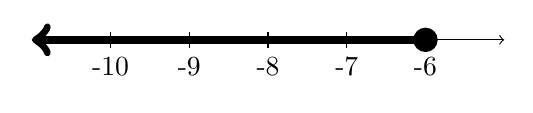
\begin{tikzpicture}
            % Draw the number line
            \draw[<->] (-11,0) -- (-5,0);
            \foreach \x in {-10,-9,-8,-7,-6}
            \draw (\x, 0.1) -- (\x, -0.1) node[below] {\x};

            % Draw the closed circle at 2
            \draw[fill=black, thick] (-6,0) circle (4pt);

            % Draw the line segment between the two points
            \draw[black, line width=3pt, <-] (-11,0) -- (-6.1,0);        \end{tikzpicture}
            \rule[-8pt]{0.75pt}{8ex} \: \raisebox{-4pt}{\framebox[36mm]{\rule{0pt}{10mm}}} \: \rule[-8pt]{0.75pt}{8ex} \: \raisebox{-4pt}{\framebox[36mm]{\rule{0pt}{10mm}}}            
    % DONE 11 ^ 
    \vspace{0.5cm}
    \item 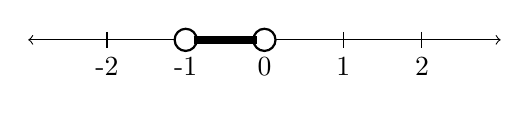
\begin{tikzpicture}
            % Draw the number line
            \draw[<->] (-3,0) -- (3,0);
            \foreach \x in {-2,-1,0,1,2}
            \draw (\x, 0.1) -- (\x, -0.1) node[below] {\x};

            % Draw the open circle at -1
            \draw[fill=white, thick] (-1,0) circle (4pt);
            % Draw the closed circle at 2
            \draw[fill=white, thick] (0,0) circle (4pt);

            % Draw the line segment between the two points
            \draw[black, line width=3pt] (-0.9,0) -- (-0.1,0);        \end{tikzpicture}
            \rule[-8pt]{0.75pt}{8ex} \: \raisebox{-4pt}{\framebox[36mm]{\rule{0pt}{10mm}}} \: \rule[-8pt]{0.75pt}{8ex} \: \raisebox{-4pt}{\framebox[36mm]{\rule{0pt}{10mm}}}            
    % DONE 12 ^ 
    \vspace{0.5cm}
    \item 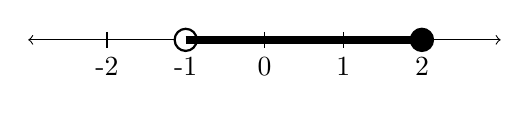
\begin{tikzpicture}
            % Draw the number line
            \draw[<->] (-3,0) -- (3,0);
            \foreach \x in {-2,-1,0,1,2}
            \draw (\x, 0.1) -- (\x, -0.1) node[below] {\x};

            % Draw the open circle at -1
            \draw[fill=white, thick] (-1,0) circle (4pt);
            % Draw the closed circle at 2
            \draw[fill=black, thick] (2,0) circle (4pt);

            % Draw the line segment between the two points
            \draw[black, line width=3pt] (-1,0) -- (2,0);        \end{tikzpicture}
            \rule[-8pt]{0.75pt}{8ex} \: \raisebox{-4pt}{\framebox[36mm]{\rule{0pt}{10mm}}} \: \rule[-8pt]{0.75pt}{8ex} \: \raisebox{-4pt}{\framebox[36mm]{\rule{0pt}{10mm}}}            
    % DONE 13 ^ 
    \vspace{0.5cm}
    \item 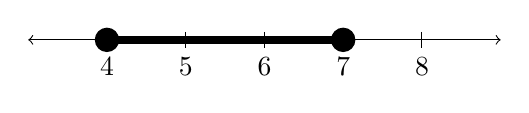
\begin{tikzpicture}
            % Draw the number line
            \draw[<->] (3,0) -- (9,0);
            \foreach \x in {4,5,6,7,8}
            \draw (\x, 0.1) -- (\x, -0.1) node[below] {\x};

            % Draw the open circle at -1
            \draw[fill=black, thick] (4,0) circle (4pt);
            % Draw the closed circle at 2
            \draw[fill=black, thick] (7,0) circle (4pt);

            % Draw the line segment between the two points
            \draw[black, line width=3pt] (4,0) -- (7,0);        \end{tikzpicture}
            \rule[-8pt]{0.75pt}{8ex} \: \raisebox{-4pt}{\framebox[36mm]{\rule{0pt}{10mm}}} \: \rule[-8pt]{0.75pt}{8ex} \: \raisebox{-4pt}{\framebox[36mm]{\rule{0pt}{10mm}}}            
    % DONE 14 ^ 
    \vspace{0.5cm}

\end{enumerate}

\end{document}